\subsection*{DRL Training Convergence Curves}
\phantomsection
\addcontentsline{toc}{subsection}{DRL Training Convergence Curves}

\noindent
Figure~\ref{fig:ppo-appendix} shows the episode reward trajectory during
Proximal Policy Optimisation (PPO) training for method M3.
The agent was trained for up to 2\,000 episodes with an early-stopping
criterion (improvement $< 0.005$ over a 100-episode window). Training
converged after approximately 250 episodes, reaching a plateau around an
episode reward of 38--40.

\begin{figure}[h]
    \centering
    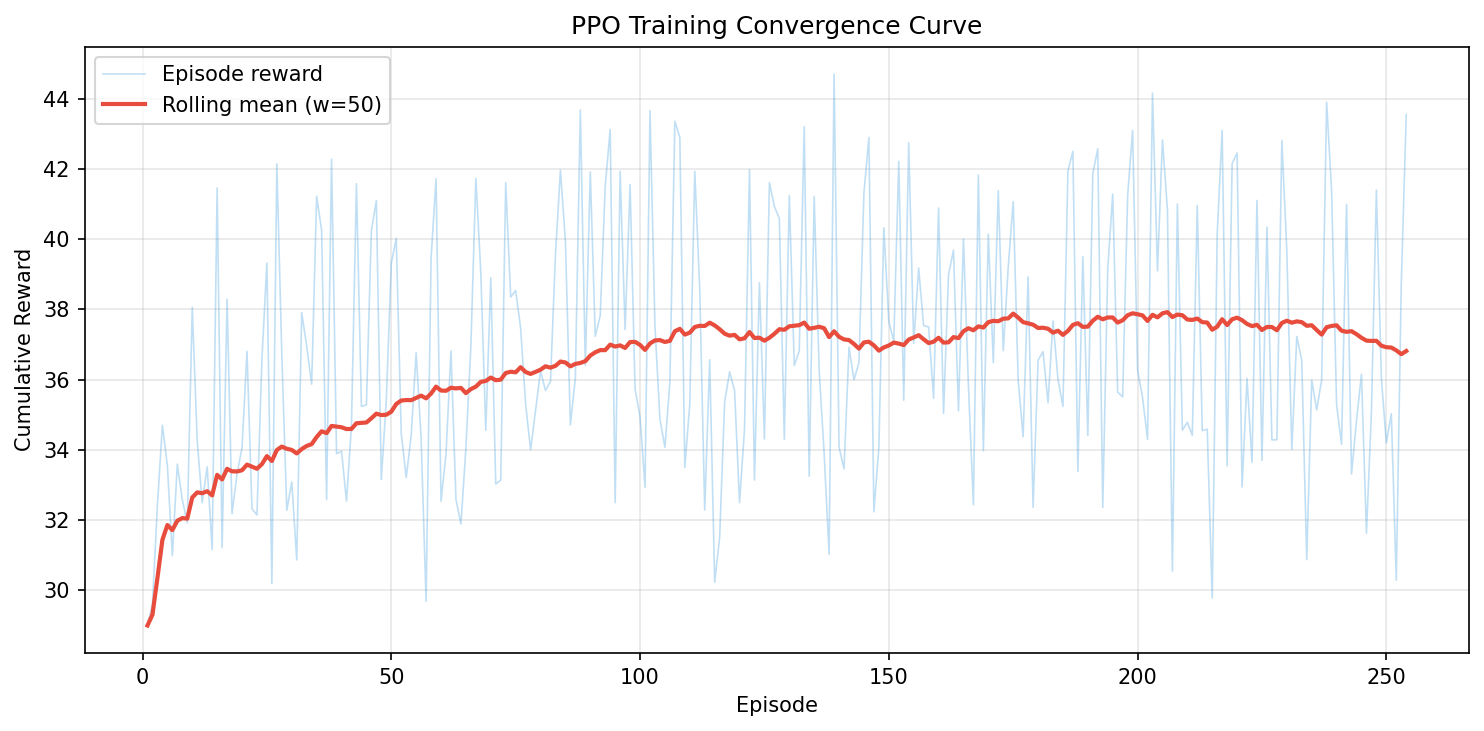
\includegraphics[width=0.85\textwidth]{figures/ppo_training_curve.png}
    \caption{PPO training curve: episode reward versus training episode. The
    shaded region indicates $\pm 1$ standard deviation computed over a
    rolling window. Training was performed with seed 42, learning rate
    $3 \times 10^{-4}$, 1\,024 rollout steps, batch size 64, and 10 PPO
    epochs per update.}
    \label{fig:ppo-appendix}
\end{figure}
